\subsection{Efficient Computation of Visibility Polygons \cite{DBLP:journals/corr/BungiuHHHK14}}
This paper \cite{DBLP:journals/corr/BungiuHHHK14} introduces new implementations and their experimental evaluations for two existing algorithms (\cite{joe1987corrections}, \cite{asano1985efficient}) and a newly developed one for computing visibility in polygons. These implementations are available in the CGAL library\footnote{\url{https://www.cgal.org/}}, starting with version 4.5.

Working with the visibility region is a basic tool in computational geometry, specifically in the Art Gallery Problem \cite{o1987art}. As the Art Gallery Problem \cite{o1987art} is an $\exists \mathbb R$-complete problem \cite{abrahamsen2021art}. The problem class $\exists \mathbb R$ consists of instances that can be reduced in polynomial time to a decision problem of whether a system of polynomial equations with integer coefficients and any number of real variables has a solution. Since NP $\subseteq \exists \mathbb R$, the $\exists \mathbb R$ class is an even harder to solve complexity class, since $\exists \mathbb R$ problems do not admit solutions in polynomial time. For this reason, it is crucial that the computation time of the visibility region is efficiently implemented. 

Therefore, this paper presents 3 algorithms and their implementations' performance.

\subsubsection{Algorithm of Joe and Simpson \cite{joe1987corrections}}
The algorithm of Joe and Simpson \cite{joe1987corrections} runs in $O(n)$ time and space. It begins by sequentially scanning the boundaries of the simple polygon $\mathcal P$, and adds its boundary points $v_i, \forall i = \overline{1, n}$, with $n$ the number of vertices in $\mathcal P$, to a stack $s$. For each processed edge $\overline{v_iv_{i + 1}}$, its endpoints $v_i$ and $v_{i + 1}$ are checked whether they are in the visibility region of the viewpoint $p$. If they are, $v_i$ and $v_{i + 1}$ are added to $s$. Otherwise, they are scanned, but not added to $s$. At every moment, the algorithm checks whether $\overline{v_iv_{i + 1}}$ obscures a previously added line segment. If that is the case, than the endpoints of the obscured line segment are declared obsolete and deleted. 

% The implementation of the algorithm handles the previously discussed cases for an arrangement $\mathcal P$, while also accounting for the case in which the polygon winds more than 360$^\circ$ using a winding counter.
% - **Algorithm of Joe and Simpson** $O(n)$ time and space
	% - performs a sequential scan of the boundary of $\mathcal P$ and uses a stack $s$ of boundary points $s_0, s_1, ..., s_ as summarised in the following subsections.der to deal with cases in which the polygon winds more than 360*, a winding counter is used during this edge processing
% he points that are visible from $q$ form the visibility region $\mathcal V(q)$ (polygon)

\subsubsection{Algorithm of Asano \cite{asano1985efficient}}
The algorithm of Asano \cite{asano1985efficient} runs in $O(n \log n)$ time and $O(n)$ space and uses a plane sweep approach with event line $L$. It begins by efficiently sorting all the vertices of $\mathcal P$ based on their polar angles with respect to the viewpoint $p$. For example, suppose $p$ and some given points $a_1, a_2, b_1, b_3$ are given in a plane with positive coordinates, as placed in Figure \ref{fig:asano}. Then, they will be treated in the order of $b_2, b_1, a_2, a_1$ with respect to $p$ and their angular comparisons $\measuredangle b_2Oq < \measuredangle b_1Oq < \measuredangle s_1Oq < \measuredangle a_1Oq$, where $O(0, 0)$. Then, the event line $L$ starts sweeping around $p$. Every line segment that $L$ intersects is stored in a balanced binary tree $T$ in the order of intersection. As $T$ is updated, a new vertex of $\mathcal V(p)$ is stored each time the segment closest to $p$ in $T$ changes. It is important to mention that the intersection between $L$ and line segments is not explicit, but is instead determined by comparisons between the endpoints' coordinates. For instance, in Figure \ref{fig:asano}, the endpoint $b_2$ of line segment $\overline{b_2a_2}$ is the first one $L$ intersects. $b_2$ is thus added into $T$. Then, $L$ continues sweeping and adds $b_1, a_2$ and $a_2$ are added into $T$. Although $\overline{b_2a_2}$ and $\overline{b_1a_1}$ represent line segments $s_2$ and $s_1$, respectively, the intersection of $L$ with them is not explicitly computed, but is determined based solely on the positions of their endpoints: $s_1$ is farther away from $p$ because $q, a_2$ and $b_2$ are on the same side of $s_2$.

\begin{figure}[h!]
	\centering
	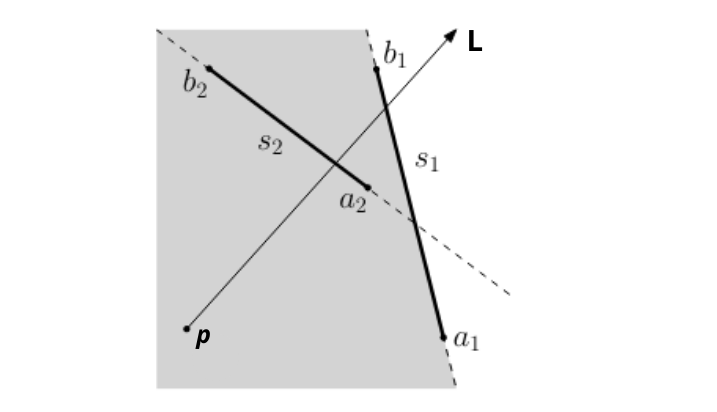
\includegraphics[width = 0.5\textwidth]{Screenshot from 2022-01-28 12-07-50.png}
	\caption{The Algorithm of Asano \cite{asano1985efficient} Example}
	\label{fig:asano}
\end{figure}
	% - as the sweep proceeds, $T$ is updated and a neq vertex of $V(q)$ is generated each time the smallest element (segment closest to $q$) in $T$ changes
	% - important to have efficient comparison ops (e.g.: *add pic*)

\subsubsection{New Algorithm: Triangular Expansion}
The algorithm introduced in the paper is called Triangular Expansion and runs in $O(n^2)$ time and $O(n)$ space. It begins by triangulating $\mathcal P$ in $O(n \log n)$ time if $\mathcal P$ has holes (it has both internal and external boundaries), and $O(n)$ otherwise. Unfortunately the implementation is constrained by CGAL, which implements the Delaunay triangulation algorithm \cite{delaunay1934sphere} in $O(n^2)$ for the worst case, but with better performance in practice. 

Figure \ref{fig:triangular} depicts an example run of the algorithm on a polygon with holes $\mathcal P$. Starting from the viewpoint $p$, the triangle containing $p$ is located by performing a simple walk. Trivially, $p$ sees the entire triangle it is contained in. The algorithm continues by recursively expanding the view of $p$ from one triangle into the other recursively. The view of $p$ becomes restricted by the reflex vertices $l$ and $r$ of the third triangle the recursive step entered through. Since $l$ and $r$ are reflex vertices, then the view past them is further restricted until the boundaries $l'$ and $r'$, respectively, of $\mathcal P$ are reached. Line segments $\overline{ll'}$ and $\overline{rr'}$ are added to $\mathcal V(p)$ in their angular order around $p$. 

\begin{figure}[h!]
	\centering
	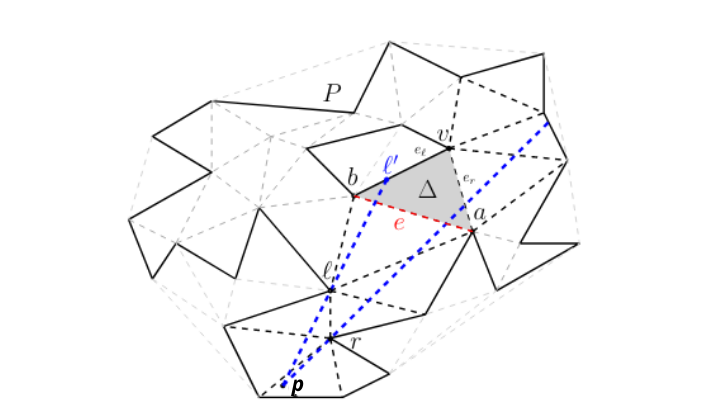
\includegraphics[width = 0.5\textwidth]{Screenshot from 2022-01-28 13-01-29.png}
	\caption{The Triangular Expansion Algorithm Example - recursion entering triangle $\Delta$ through edge $e$.}
	\label{fig:triangular}
\end{figure}
% - **triangular expansion** - $O(n^2)$
	% - preprocessing: triangulation ($O(n)$ for simple polygons, $O(n\log n$) for polygons with holes; Delaunay ($O(n^2)$) used)
	% - given $q$, locate the triangle containing $q$ by a simple walk ($q$ sees the entire triangle)
	% - recursive procedure that expands the view of $q$ through that edge into the next triangle. Initially, the view is restricted by the 2 endpoints of the edge, and then further as recursion continues: *add pic* for triangle $\Delta$, the view of $q$ is restricted by the 2 reflex vertices $l$ and $r$ with $a \leq r < l \leq b$ w.r.t. angular order around $q$. $v$ is a new vertex and its position w.r.t. $l$ and $r$ is computed with 2 orientation tests *add pic*: $e_l$ is a boundary edge and we can report edge $\overline{ll'}$ and $\overline{l'v}$ as part of the visibility region of $q$; $e_r$ is not a boundary edge => the recursion continues with $v$ being the vertex that now restricts the left side of the view
	% - the recursion may split into 2 calls if $e_l$ and $e_r$ are both not part of the boundary. As there are $n$ vertices, this can happen $O(n)$ times => worst-case $O(n^2)$; however a true split into two visibility cones that may reach the same triangle independently can only happen at a hole of $\mathcal P$, thus at worst the runtime is $O(nh)$, where $h$ = number of holes (linear time of simple polygons) (e.g.: worst-case *add pic*)
	% - triangulation has linear size, at most $O(n)$ recursive calls on the stack => $O(n)$ space

\subsubsection{Experiments}
The paper does not report on benchmarks with query points on edges in the interior polygon, as it claims that the implementations perform similarly to other already implemented algorithms. Instead, it uses two real-world scenarios (a simple polygon of Norway with 20981 vertices, and a cathedral polygon with 1209 vertices) and a worst-case polygon for the Triangular Expansion algorithm.

In terms of results on the real-world polygons, the Triangular Expansion algorithm has a 2-factor improved performance when compared to Asano's algorithm \cite{asano1985efficient}, and performs one order of magnitude faster than Joe and Simpson's algorithm \cite{joe1987corrections}. For the worst-case scenario, Asano's algorithm \cite{asano1985efficient} outperforms the Triangular Expansion algorithm with increasing input complexity.

Thus, despite the Triangular Expansion algorithm being outperformed in the worst-case scenario, this paper introduces efficient implementations for the 3 different visibility polygon algorithms in the CGAL library. The choice of algorithms when using the library can be adapted based on the input polygons. 
% - experiments - no reports on similar benchmarks with query points on edges and in the interior polygon; for the input graphs used, the triangular expansion is 2-factor faster than Asano, and one order of magnitude faster than Joe and Simpson; with increasing input complexity, Asano does become faster